\chapter{Analýza a návrh řešení}
Tato kapitola pojednává o analýze a návrhu vhodného řešení aplikace. Výstupem této analýzy jsou funkční a nefunkční požadavky. Dále návrh a popis domén a nejdůležitější případy užití s aktéry. 

\section{Požadavky}
Požadavky na systém se dělí na dvě sekce obecné a funkční požadavky. Pro definování těchto požadavků jsem vycházel z oficiálního zadání práce. Tyto požadavky mi definují návrh aplikace a později ve fázi implementace i potřebné technologie pro implementaci systému.
\subsection{Obecné požadavky}
Obecné požadavky se netýkají funkčnosti, ale celkového návrhu a použitých technologií.
\begin{enumerate}
\item Systém bude postaven na webovém frameworku Ruby on Rails.
\item Systém bude používat databázi MySQL.
\item Systém bude webovou aplikací.
\item Serverová část systému poběží na aplikačním serveru Apache HTTP server.
\item Systém bude používat webovou službu KOSapi.
\item Systém bude pro autentizaci používat FELid.
\end{enumerate}

\subsection{Funkční požadavky}
Tato sekce se zabývá požadavky na funkčnost systému.
\begin{enumerate}
\item Systém umožní spravovat uživatele.
\item Systém umožní průběžné plánování hospitaci.
\item Systém umožní hospitujícímu i hospitovanému prohlížet hospitace.
\item Systém umožní vystavit závěrečné hodnocení na veřejné části aplikace. 
\item Systém umožní hospitovanému sepsat stanoviska k názorům hospitujícího.
\item Systém umožní hospitujícímu nahrát naskenovaný dokument hodnocení výuky.
\item Systém umožní hospitujícímu napsat slovní hodnocení z výuky.
\item Systém umožní hospitujícímu napsat závěrečné shrnutí hospitace.
\item Systém bude odesílat emailem zprávy o naplánování hospitací a jednotlivé hodnocení a stanoviska příslušným osobám.
\item Systém umožní vyhledávat předměty z KOSapi.
\item Systém umožní vyhledávat osoby z KOSapi.
\end{enumerate}

\section{Uživatelské role}
V systému je celkem 6 uživatelských rolí, ty jsou odvozeny z modelu aktérů na obrázku \ref{fig:actors}. Máme tři základní uživatelské role, které jsou základem systému - přihlášený uživatel, nepřihlášený uživatel a administrátor hospitací. Další role jako hospitovaný a hospitující uživatel jsou přiděleny příslušným osobám zainteresovaných v jednotlivých hospitacích.

\begin{figure}[h]
\begin{center}
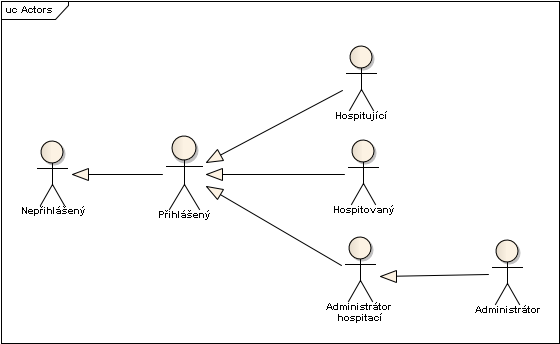
\includegraphics[width=16cm]{figures/Actors}
\caption{Aktéři}
\label{fig:actors}
\end{center}
\end{figure}

V systému jsou následující role:

\subsection{Nepřihlášený uživatel}
Nepřihlášený uživatel je role pro hosty naší aplikace. V systému má ze všech rolí nejmenší pravomoc. V tomto stavu je každý uživatel, který se doposud nepřihlásil do systému a je mu umožněno vykonat následující akce. Přihlásit se, zobrazit seznam naplánovaných veřejných hospitací na aktuální a následující semestr. Má také přístup k závěrečným shrnutím hospitací.

\subsection{Přihlášený uživatel}
Přihlášený uživatel dědí z role nepřihlášeného uživatele. Je to uživatel, který má vytvořený účet v systému a již se přihlásil. Tato role přidává možnost odhlásit se a procházet veškeré ohlášené hospitace. Tato role je základní pro všechny další role a z ní taky dědí.

\subsection{Hospitovaný}
Hospitovaný je role pro přihlášeného uživatele v systému. Je přidělená pro každého vyučujícího, který vyučuje předmět, na němž byla naplánovaná hospitace. Tato role přidává možnost přístupu k naplánovaným hospitacím, kde figuruje jako hospitovaný. U těchto hospitací má právo na zobrazení všech hodnotících dokumentů a umožní mu sepsat dokument se stanovisky k názorům hospitujícího.

\subsection{Hospitující}
Hospitující je role pro přihlášeného uživatele v systému. Přiděluje ji administrátor hospitací osobám, které mají za úkol vykonat hospitaci. U přidělených hospitací má uživatel právo na zobrazení informací o jeho hospitaci a povinnost sepsat hodnotící dokumenty z vykonané hospitace.

\subsection{Administrátor hospitací}
Tato role patří mezi nejdůležitější role v systému, protože spravuje hospitace a přiděluje uživatelům nové role. Hlavním účelem této role je plánovat hospitace na předměty a posléze je spravovat.   

\subsection{Administrátor}
Administrátor je super uživatel, který má nejvyšší pravomoc v systému. Má přístup ke všem zdrojům aplikace a může nastavovat aplikaci.

\section{Doménový model}
Doménový model na obrázku \ref{fig:domainmodel} reprezentuje klíčové domény systému a jejich vztahy mezi sebou. 

Popis domény jsem pro přehlednost rozdělil podle zdroje na dvě základní skupiny. V první skupině jsou domény, které používám z KOSapi a druhou skupinou jsou domény specifické pro moji aplikaci. 

\subsection{Domény z KOSapi}
\begin{itemize}
\item Osoba - informace o osobě nacházející se na FEL. Každá osoba může být učitelem a studentem.
\item Semestr - informace o jednotlivých semestrech. 
\item Předmět - popis jednotlivých předmětů vyučovaných na FEL.
\item Instance předmětu - jsou instance předmětu vypsané v konkrétním semestru.
\item Paralelka - je vypsaná rozvrhová paralelka pro instanci předmětu.
\item Místnost - informace o místech, kde probíhá výuka předmětů
\end{itemize}

\subsection{Domény aplikace}
\begin{itemize}
\item Uživatel - obsahuje dodatečné informace a role pro osobu v aplikaci.
\item Hospitace - obsahuje informace o naplánování hospitace. 
\item Poznámka - je textová poznámka pro hospitaci napsaná uživatelem.
\item Příloha - je připojený datový soubor k hodnocení hospitace.
\item Formulář - je vyplněný formulář pro hospitaci.
\item Hodnota - je vyplněná hodnota jedné formulářové položky.
\item Typ formuláře - udává formát dokumentu, který se používá pro hospitace. 
\item Položka - je šablona jedné položky ve formuláři.
\end{itemize}

\begin{figure}[p]
\begin{center}
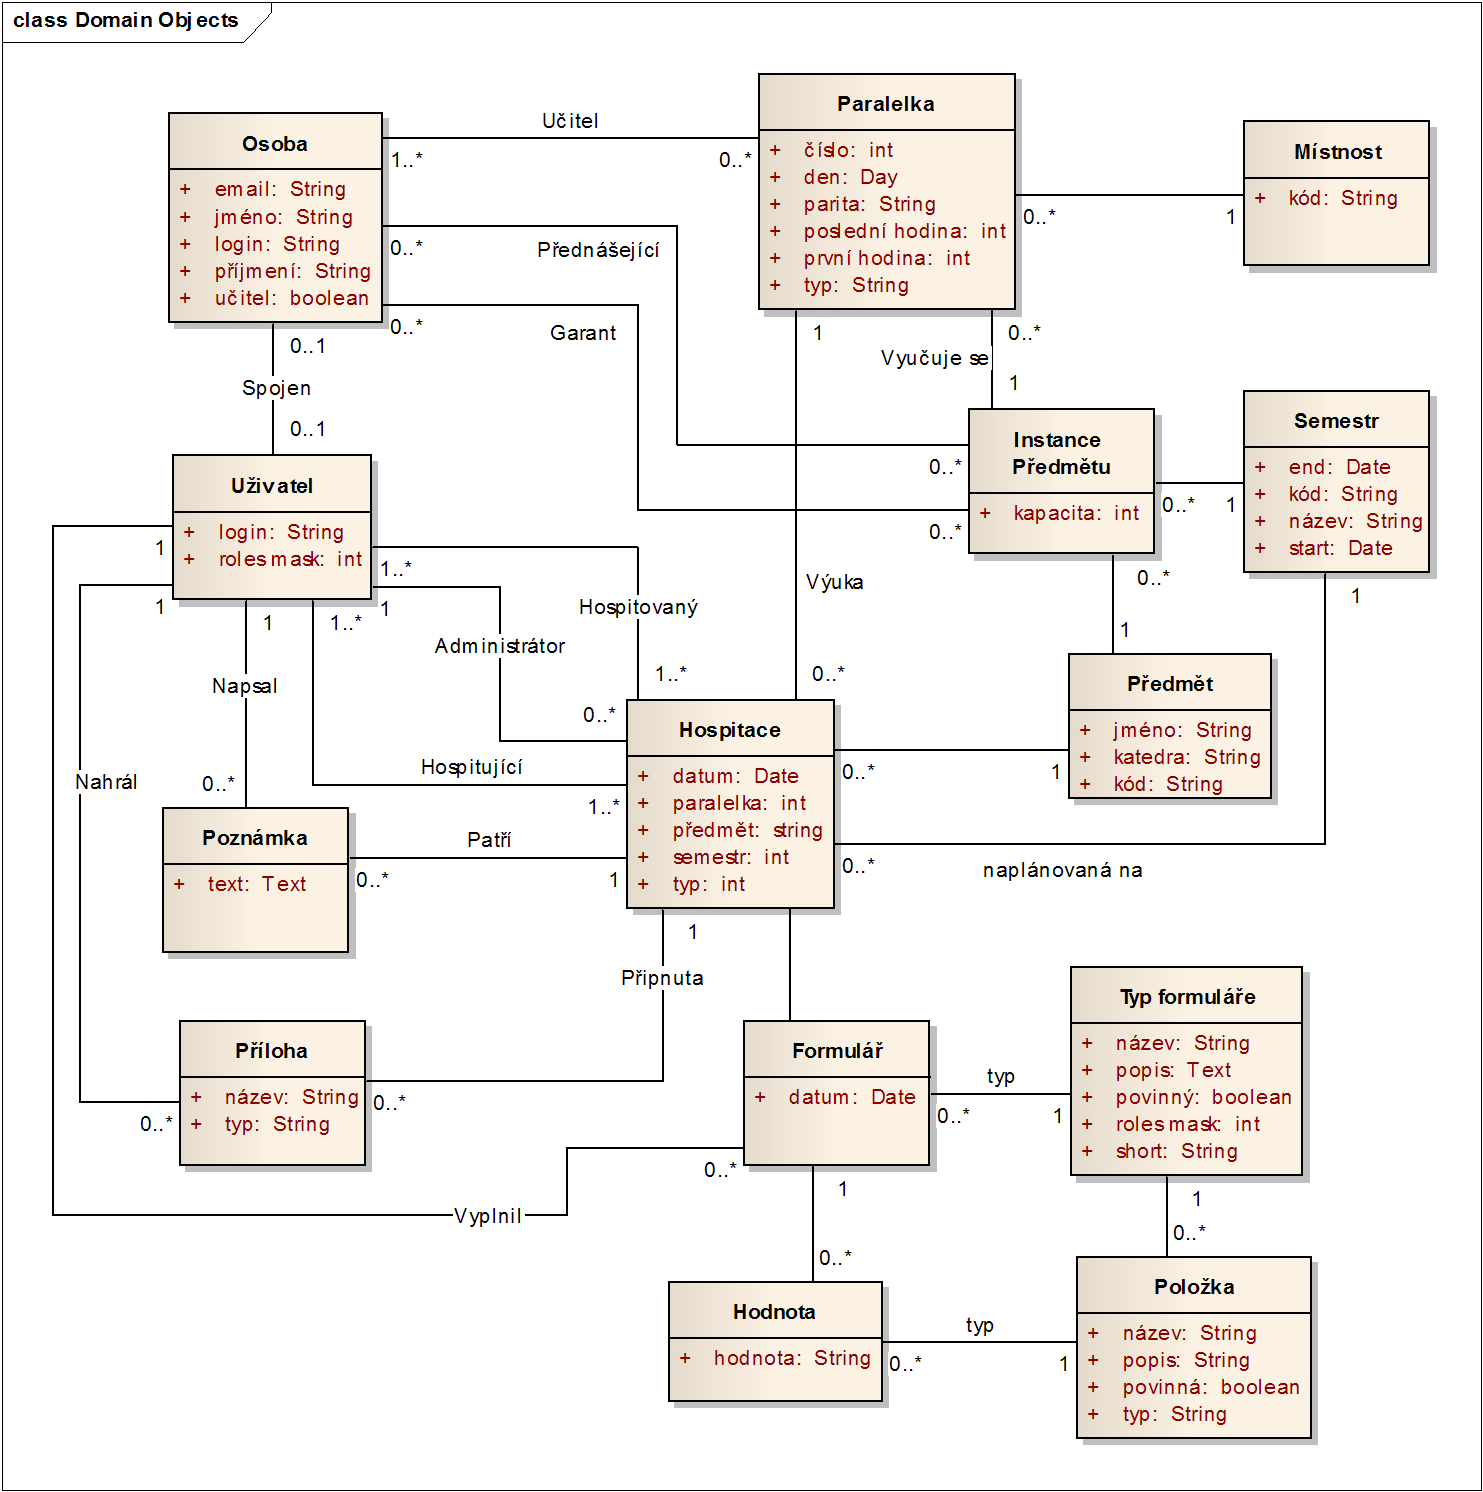
\includegraphics[width=16cm]{figures/DomainModel}
\caption{Doménový model}
\label{fig:domainmodel}
\end{center}
\end{figure}

\section{Životní cyklus hospitace}
Cílem této části analýzy je popsat životní cyklus, kterým hospitace prochází. 

\subsection{Vytvoření}
Životní cyklus hospitace začíná jejím vytvářením. Toto zajišťuje administrátor hospitací. Ten založí hospitaci pro kterou definuje semestr, kdy se má hospitace uskutečnit a předmět vyučovaný na fakultě. Při vytváření hospitace se určí typ hospitace a tím i její způsob zviditelnění, pro ostatní aktéry v aplikaci.

\subsection{Naplánování}
V této fázi je také hlavním aktérem administrátor hospitace. V této části životního cyklu administrátor určí hospitovanou paralelku předmětu a datum,  kdy se hospitace uskuteční.  

Administrátor také v této fázi přidělí hospitující z řad pedagogů určených k vykonání hospitace.  
 
\subsection{Hodnocení}
Poté, co proběhla kontrola hospitace, začíná nová fáze, ve které se hodnotí vyučování. Do této fáze už nezasahuje aktér administrátor hospitace. Za to přicházejí na scénu dva aktéři hospitovaný a hospitující.

V první fázi musí hospitující vyplnit, nebo nahrát naskenovaný formulář pro Hodnocení výuky při hospitaci. Tento formulář slouží k dokumentaci průběhu hospitace.

V druhé fázi jeden z hospitujících sepíše slovní hodnocení hospitační návštěvy.

Ve třetí fázi může hospitovaný do dvou dnů vyplnit stanovisko hodnoceného k názorům hospitujícího.  

V poslední fázi jeden z hospitujících sepíše poslední formulář Závěrečné shrnutí. Po vyplnění tohoto formuláře se hospitace stává ukončenou a tím končí její životní cyklu.
 
\section{Technologie}
Tato část popisuje jednotlivé technologie potřebné pro implementaci aplikace.

\subsection{Ruby on Rails}
Ruby on Rails, zkráceně Rails, je jedno z implementačních omezení, které se nachází přímo v zadání práce. Je to framework postavený na jazyce Ruby a je primárně určen pro tvorbu webových aplikací napojených na databázi. Rails je postaven na návrhovém vzoru model-view-controller. Tento framework používá dva hlavní principy. Prvním principem je Convention over Configuration a druhým je Don’t Repeat Yourself.

\subsection{KOSapi}
KOSapi je webová služba poskytující aplikační rozhraní v podobě RESTful webové služby. Tato služba je určená pro vznik školních aplikací, které potřebují mít přístup k datům souvisejícím s výukou. Tato služba čerpá data z KOSu pro instance FEL a FIT.

Z této služby čerpám hlavně data předmětů a osob v KOSu. Pro připojení ke KOSapi jsem rozšířil již existující knihovnu napsanou v Ruby pány Tomášem Linhartem a Tomášem Jukínem ve školním projektu VyVy. 

\subsection{FELid}
FELid je globální autentizační a autorizační systém pro webovské aplikace na síti FEL. Poskytuje jednotný a bezpečný způsob přihlášení uživatelů a přenos jejich údajů do různých aplikací na webu. Zároveň podporuje jednorázové přihlášení (tzv. single sign-on). Znamená to, že se uživatel přihlašuje pouze do první použité aplikaci a u dalších aplikací už nemusí zadávat svoje přihlašovací údaje.

Tuto službu používám pro autentizaci uživatelů do systému. Abych mohl používat v aplikaci FELid je nutné splnit technické požadavky, které jsou napsány na stránkách FELid.

\subsection{Aplikační server}
Pro zprovoznění aplikace do reálného provozu jsem použil webový server Apache HTTP server ve verzi 2. Tato verze webového serveru totiž umožňuje instalaci zásuvných modulů Passenger a Shibboleth. Passenger umožňuje nasazení rails aplikací na serveru. Druhý modul Shibboleth zprostředkovává single sign-on autentizaci mezi aplikací a službou FELid.

\subsection{Databáze}
Ruby on Rails poskytuje možnost připojení k různým databázovým systémům prostřednictvím adaptérů. Díky tomu není aplikace závislá na použitém databázovém systému a díky tomu mohu používat pro vývoj a testování aplikace jednoduchý databázový systém SQLite, který pro tyto účely bohatě postačuje a není potřeba jej složitě konfigurovat. Pro samotné nasazení aplikace do provozu už používám databázový systém MySQL.

\section{Architektura}
V této části popisuji architektonické vzory a konvence používané pro vývoj aplikace. 

\subsection{MVC}
MVC (Model-view-controller) je softwarová architektura, která rozděluje datový model aplikace, uživatelské rozhraní a řídicí logiku do tří nezávislých komponent tak, že modifikace některé z nich má minimální vliv na ostatní. 

Ruby on Rails obsahuje ve svém jádru tuto architekturu, proto je její implementace automatická.

\subsection{DRY}
DRY (Don’t repeat yourself) je princip vývoje softwaru zaměřený na snížení opakování psaní stejného kódu a tím zvyšuje čitelnost a znovupoužitelnost kódu. To znamená, že informace se nacházejí na jednoznačném místě. Pro příklad Ruby on Rails získává definici sloupců pro třídu modelu přímo z databáze.  

\subsection{CoC}
CoC (Convention over Configuration) je další princip používaný v Rails pro zlepšení čitelnosti a znovupoužitelnosti kódu. Tento princip znamená, že konvence má přednost před konfigurací a to tak že Rails předpokládá to, co chcete udělat, místo toho aby vás nutil specifikovat každou drobnost v konfiguraci. 

\subsection{REST}
REST (Representational State Transfer) je architektonický vzor pro webové aplikace. Je založen na HTTP protokolu a hlavní myšlenkou je poskytovat přístup ke zdrojům dat. Všechny zdroje jsou identifikovány přes URI. REST definuje čtyři základní metody pro přístup ke zdrojům. Jde o metody POST, GET, PUT a DELETE, které zprostředkovávají základní operace create, read, update a delete.
